\chapter{Recommender systems}
[DEPRECATED; BORROWED FROM 6.390 COURSE NOTES, NOT WRITTEN BY SHAUNTICLAIR RUIZ]

The problem of choosing items from a large set to recommend to a user
comes up in many contexts, including  music services, shopping, and online
advertisements.  As well as being an important application, it is
interesting because it has several formulations, some of which take
advantage of a particular interesting structure in the problem.  

Concretely, we can think about a company like Netflix, which
recommends movies to its users.  Netflix knows the ratings given by
many different people to many different movies, and knows your ratings on a
small subset of all possible movies. How should it use this data to 
recommend a movie for you to watch tonight?

There are two prevailing approaches to this problem.  The first,
{\em content-based recommendation}, is formulated as a supervised learning
problem.  The second, {\em collaborative filtering}, introduces a new
learning problem formulation.

\section{Content-based recommendations}
In content-based recommendation, we try to learn a predictor, $f$,
that uses the movies that you have rated so far as training data,
find a hypothesis that maps a movie into a prediction of what rating
you would give it, and then return some movies with high predicted
ratings.  

The first step is designing representations for the input and output.

It's actually pretty difficult to design a good feature representation
for movies.   Reasonable approaches might construct features based on
the movie's genre, length,  main actors, director, location, or even
ratings given by some standard critics or aggregation sources.  This
design process would yield
    \[\phi : \text{movie} \rightarrow \text{vector}\;\;.\]

Movie ratings are generally given in terms of some number of stars, 
so the output domain might be \{1, 2, 3, 4, 5\}.  It's not
appropriate for one-hot encoding on the output, and pretending that
these are real values is also not entirely sensible.  Nevertheless, we
will treat the output as if it's in $\R$.
\note{Thermometer coding might be reasonable, but it's hard to say
  without trying it.  Some more advanced techniques try to predict
  rankings (would I prefer movie A over movie B) rather than raw
  ratings.} 
\question{What is the disadvantage of using one-hot?
  What is the disadvantage of using $\R$?}

Now that we have an encoding, we can make a 
training set based on {\em your} previous ratings of movies. Here,
$\ex{x}{i}$ represents the $i$th movie, $\phi(\ex{x}{i})$ gives our 
feature representation of the $i$th movie, and $\ex{y}{i} = \text{rating}(\ex{x}{i})$
is your rating for the $i$th movie. If we let $J = \{1,2, \ldots, j\}$ be the index set of all movies that you have rated so far,
the resulting training set looks like
    \[ D_a = \left\{
        \left(\phi(\ex{x}{1}), \text{rating}(\ex{x}{1})\right),
        \left(\phi(\ex{x}{2}), \text{rating}(\ex{x}{2})\right),
        \ldots,
	\left(\phi(\ex{x}{j}), \text{rating}(\ex{x}{j})\right)
      \right\}\;\;.\]

The next step is to pick a loss function.  This is closely related to
the choice of output encoding.  Since we decided to treat the output
as a real, we can formulate the problem as a  regression from $\phi
\rightarrow \mathbb{R}$, with $\text{Loss}(p, y) = \frac{1}{2}(p-y)^2$
We will generally need to regularize because we typically have a very
small amount of data (unless you really watch a lot of movies!).  

Finally, we need to pick a hypothesis space.  The simplest thing would
be to make it linear, but you could definitely use something fancier,
like a neural network.  

If we put all this together,  with  a linear hypothesis space, we end
up with the objective
    \[J(\theta) = \frac{1}{2}\sum_{i \in J}
      (\theta^T \phi( \ex{x}{i} ) + \theta_0 - \ex{y}{i})^2
      + \frac{\lambda}{2} \norm{\theta}^2\;\;.\]
      This is our old friend, ridge regression, and can be solved
      analytically or with gradient descent.

\section{Collaborative filtering}
There are two difficulties with content-based recommendation systems:
\begin{itemize}
\item It's hard to design a good feature set to represent movies.
\item They only use your previous movie ratings, but don't have a way
  to use the vast majority of their data, which is ratings from other
  people. 
\end{itemize}
In collaborative filtering, we'll try to use {\em all} the ratings
that other people have made of movies to help make
better predictions for you.  

Intuitively, we can see this process as finding the kinds of people
who like the kinds of movies you like, and then predicting that you will
like other movies that they like.
\note{In fact, there's a third strategy that is really directly based
  on this idea, in which we concretely try to find other users who are
  our  ``nearest neighbors'' in movie preferences, and then predict
  movies they like.  The approach we discuss here has similar
  motivations but is more robust.}

Formally, we will start by constructing a \note{We will in fact not
  {\em actually} represent the whole data matrix explicitly---it would
  be too big.  But it's useful to think about.}  {\em data matrix}
$Y$, where $Y_{ai}$ represents the score given by user $a$ to movie
$i$. So, if we have $n$ users and $m$ movies, $Y$ has shape
$n \times m$.

\begin{center}
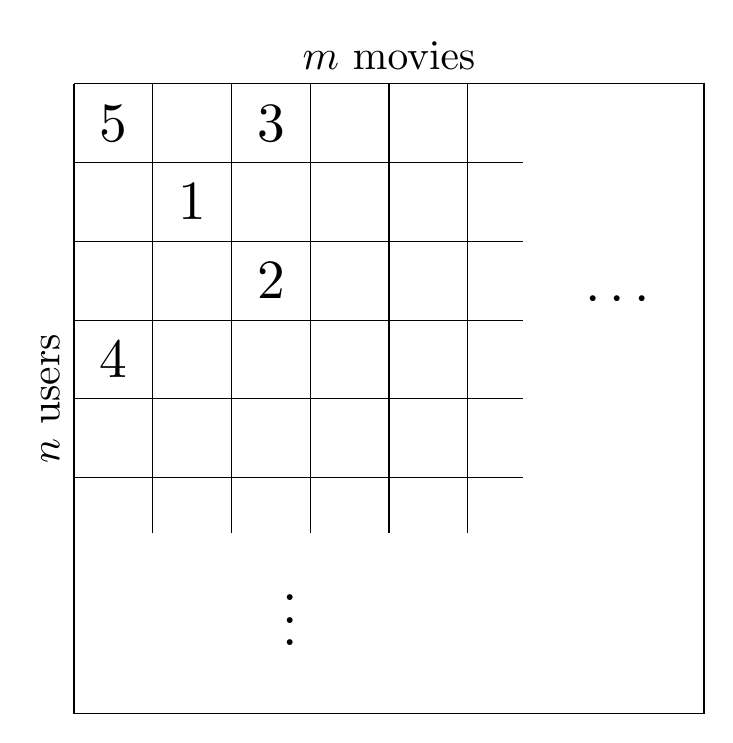
\begin{tikzpicture}
\draw (0, 0) -- (8, 0) -- (8,-8) -- (0, -8) -- (0, 0);
\foreach \y in {1,2,3,4,5}
{
\draw (0,-\y) -- (5.7,-\y);
}
\foreach \x in {1,2,3,4,5}
{
\draw (\x,0) -- (\x,-5.7);
}
\node[scale=2] (vdots) at (2.75, -6.6) {$\vdots$};
\node[scale=2] (vdots) at (6.9, -2.75) {$\cdots$};

\node[scale=2] at (0.5, -0.5) {5};
\node[scale=2] at (2.5, -0.5) {3};
\node[scale=2] at (1.5, -1.5) {1};
\node[scale=2] at (2.5, -2.5) {2};
\node[scale=2] at (0.5, -3.5) {4};
\node[above, scale=1.5] (movies) at (4,0) {$m$ movies};
\node[rotate=90, scale=1.5, above] (users) at (0,-4) {$n$ users};
\end{tikzpicture}
\end{center}

$Y$ is very sparse (most entries are empty).  \note{In the Netflix
  challenge data set, there are 400,000 users and 17,000 movies.
  Only 1\% of the data matrix is filled.}  So, we will think of our
training data-set as a set of tuples $\left\{(a,i,r)\right\}$, 
where $a$ is the index assigned to a particular user, $i$ is the index
assigned to a particular movie, and $r$ is user $a$'s rating of movie
$i$. We will use $D = \left\{(a,i): Y_{ai} \text{ is non-empty}\right\}$ 
as the set of indices for which we have a rating.

We are going to try to find a way to use $D$ to predict values for
missing entries. Let $X$ be our predicted matrix of ratings.  Now, we
need to find a loss function that relates $X$ and $Y$, so that we can
try to optimize it to find a good predictive model.

\paragraph*{Idea \#1}
Following along with our previous approaches to designing loss
functions, we might want to say that our predictions $X_{ai}$ should
agree with our data $Y_{ai}$, and then add some regularization,
yielding loss function
\[\text{Loss}\text{}(X, Y) = \frac{1}{2} \sum_{(a,i) \in D}
(X_{ai}-Y_{ai})^2 + \sum_{\text{all } (a,i)}X_{ai}^2\;\;.\]
{\em This is a {\bf bad} idea!}  It will set $X_{ai} = 0$ for all $(a,
i) \not \in D$. 
\question{Convince yourself of that!}
We need to find a different kind of regularization that will force
some generalization to unseen entries.

\begin{examplebox}
\paragraph*{Linear algebra idea:}
The \emph{rank} of a matrix is the maximum number of linearly independent
rows in the matrix (which is equal to the maximum number of linearly
independent columns in the matrix). 

If an $n \times m$ matrix $X$ is rank 1, then there exist $U$ and $V$ of
shapes $n \times 1$ and $m \times 1$, respectively, such that
\[X = UV^T\;\;.\]
If $X$ is rank $k$, then there exist $U$ and $V$ of shape $n \times k$
and $m \times k$, respectively, such that
\[X = UV^T\;\;.\]
\end{examplebox}

\paragraph*{Idea \#2}
Find the rank 1 matrix $X$ that fits the entries in $Y$ as well as
possible.   This is a much lower-dimensional representation (it has $m
+ n$ parameters rather than $m \cdot n$ parameters) and the same
parameter is shared among many predictions, so it seems like it might
have better generalization properties than our previous idea.

So, we would need to find vectors $U$ and $V$ such that
\[
  UV^T
  = 
  \begin{bmatrix}
    \ex{U}{1} \\ \vdots \\ \ex{U}{n}
  \end{bmatrix}
  \begin{bmatrix}
    \ex{V}{1} & \cdots & \ex{V}{m}
  \end{bmatrix}
  =
  \begin{bmatrix}
    \ex{U}{1}\ex{V}{1} & \cdots & \ex{U}{1}\ex{V}{m} \\
    \vdots & \ddots & \vdots \\
    \ex{U}{n}\ex{V}{1} & \cdots & \ex{U}{n}\ex{V}{m} \\
  \end{bmatrix}
  =
  X \;\;.
\]
And, since we're using squared loss, our objective function would be
\[
  J(U,V) = \frac{1}{2}
  \sum_{(a,i)\in D}(\ex{U}{a}\ex{V}{i} - Y_{ai})^2 \;\;.
\]

Now, how can we find the optimal values of $U$ and $V$?  We could take
inspiration from our work on linear regression and see what the
gradients of $J$ are with respect to the parameters in $U$ and $V$.
For example, 
\[
  \frac{\partial J}{\partial \ex{U}{a}} = \sum_{\{i \mid (a,i) \in D\}}
  (\ex{U}{a}\ex{V}{i} - Y_{ai})\ex{V}{i} \;\;.
\]
We could get an equation like this for each parameter $\ex{U}{a}$ or
$\ex{V}{i}$.  We don't know how to get an immediate analytic solution
to this set of equations because the parameters $U$ and $V$ are
multiplied by one another in the predictions, so the model does not
have a linear dependence on the parameters.  We could approach this
problem using gradient descent, though, and we'll do that with a
related model in the next section.

But, before we talk about optimization, let's think about the
expressiveness of this model.  It has one parameter per user (the
elements of $U$) and one parameter per movie (the elements of $V$),
and the predicted rating is the product of these two.  It can really
represent only each user's general enthusiasm and each movie's general
popularity, and predict the user's rating of the movie to be the
product of these values.
\question{
What if we had two users, 1 and 2,  and two movies, A and B.  Can  you
find $U, V$ that represents the data set $(1, A, 1), (1, B, 5),
(2, A, 5), (2, B, 1)$ well?
}

\paragraph*{Idea \#3}
If using a rank 1 decomposition of the matrix is not expressive
enough, maybe we can try a {\em rank $k$} decomposition!   In this
case, we would try to find an  $n\times k$
matrix $U$ and an $m \times k$ matrix $V$ that minimize
\[J(U,V) = \frac{1}{2} \sum_{(a,i)\in D} (\ex{U}{a} \cdot \ex{V}{i}
  - Y_{ai})^2\;\;.\]

\begin{center}
  \begin{tikzpicture}[scale=1.3]
  \draw [thick] (-0.3,0) to [square left brace] (-0.3,4);
  \draw [thick] (0.7,0) to [square right brace] (0.7,4);
  \node [scale=1.6] at (0.2, 2) {$U$};

  \draw [thick] (2,0) to [square left brace] (2,4);
  \draw [thick] (6,0) to [square right brace] (6,4);

  \draw [thick] (2,4.7) to [square left brace] (2,6.2);
  \draw [thick] (6,4.7) to [square right brace] (6,6.2);
  \node [scale=1.6] at (4, 5.45) {$V^T$};

  \draw[ultra thick, blue] (-0.6, 3) rectangle (1, 3.5);
  \draw[ultra thick, red] (5, 4.7) rectangle (5.5, 6.2);
  \draw[ultra thick] (5, 3) rectangle node
    [yshift=-5ex, xshift=-2ex, scale=1.2]
    {$X_{ai} = \ex{U}{a} \cdot \ex{V}{i}$}(5.5, 3.5);
  \node [scale=1.2, left] at (-0.5, 3.25) {$\ex{U}{a}$};
  \node [scale=1.2, above] at (5.25, 6.2) {$\ex{V}{i}$};
  \draw [dotted, thick, blue] (1.2, 3.25) -- (4.8, 3.25);
  \draw [dotted, thick, red] (5.25, 4.5) -- (5.25, 3.7);
\end{tikzpicture}
\end{center}


Here, the length $k$ vector $\ex{U}{a}$ is the $a^{th}$ row of $U$,
and represents the $k$ ``features'' of person $a$. Likewise, the
length $k$ vector $\ex{V}{i}$ is the $i^{th}$ row of $V$, and 
represents the $k$ ``features'' of movie $i$. Performing the matrix
multiplication $X = UV^T$, we see what the prediction for person
$a$ and movie $i$ is $X_{ai} = \ex{U}{a} \cdot \ex{V}{i}$.

The total number of parameters that we have is $nk + mk$. But, it is
a redundant representation. We have 1 extra scaling parameter when
$k=1$, and $k^2$ extra parameters in general. So, we really effectively have
$nk + mk - k^2$ ``degrees of freedom.''
\question{Imagine $k = 3$.  If we were to take the matrix $U$ and
  multiply the first column by 2, the second column by 3 and the third
  column by 4, to make a new matrix $U'$, what would we have  to do to
  $V$ to get a $V'$ so that $U'{V'}^T = UV^T$?  How does this question
  relate to the comments above about redundancy?}

It is still useful to add offsets to our predictions, so we will
include an $n \times 1$ vector $b_U$ and an $m \times 1$ vector $b_V$
of offset parameters, and perform regularization on the parameters in
$U$ and $V$.  So our final objective becomes
\[
  J(U,V) = \frac{1}{2} \sum_{(a,i)\in D} 
           (\ex{U}{a} \cdot \ex{V}{i} + \ex{b_U}{a} + \ex{b_V}{i}
            - Y_{ai})^2
            + \frac{\lambda}{2} \sum_{a=1}^n \norm{\ex{U}{a}}^2
            + \frac{\lambda}{2} \sum_{i=1}^m \norm{\ex{V}{i}}^2
\;\;.\]
\question{What would be an informal interpretation of $\ex{b_U}{a}$?
    Of $\ex{b_V}{i}$?}

\subsection{Optimization}
Now that we have an objective, it's  time to optimize!  There are two
reasonable approaches to finding $U$, $V$, $b_U$, and $b_V$ that
optimize this objective:  alternating least squares (ALS), which builds on
our analytical solution approach for linear regression, and 
stochastic gradient descent (SGD), which we have used in the context
of neural networks and other models.

\subsubsection{Alternating least squares}
One interesting thing to notice is that, if we were to fix $U$ and
$b_U$, then finding the minimizing $V$ and $b_V$ is a linear
regression problem that we already know how to solve.  The same is
true if we were to fix $V$ and $b_V$, and seek $U$ and $b_U$.
So, we will consider an algorithm that takes alternating steps of this
form:  we fix $U, b_U$, initially randomly, find the best $V, b_V$;
then fix those and find the best $U, b_U$, etc.

This is a kind of optimization sometimes called ``coordinate
descent,''  because we only improve the model in one (or, in this
case, a set of) coordinates of the parameter space at a time.
Generally, coordinate descent has similar kinds of convergence
properties as gradient descent, and it cannot guarantee that we find a
global optimum.  It is an appealing choice in this problem because we
know how to directly move to the optimal values of one set of
coordinates given that the other is fixed.

\vspace*{0.3cm}
\noindent More concretely, we:
\begin{enumerate}
  \item Initialize $V$ and $b_V$ at random
  \item For each $a$ in $1, 2, \ldots, n$:
    \begin{itemize}
      \item Construct a linear regression problem to find $\ex{U}{a}$ and $\ex{b_U}{a}$
        to minimize
        \[\frac{1}{2}\sum_{\{i \mid (a,i) \in D\}}
          \left(\ex{U}{a}\cdot \ex{V}{i} + \ex{b_U}{a} + \ex{b_V}{i}
          - Y_{ai}\right)^2 + \frac{\lambda}{2}\norm{\ex{U}{a}}^2
        \;\;.\]
      \item Recall minimizing the least squares objective (we are
        ignoring the offset and regularizer in the following so you
        can see the basic idea):
        \[(W\theta - T)^T(W\theta - T)\;\;.\]
        In this scenario, 
        \begin{itemize}
        \item $\theta = \ex{U}{a}$ is the $k \times 1$ parameter
          vector that we are trying to find,
        \item $T$ is a $m_a \times 1$ vector of target values
        (for the $m_a$ movies $a$ has rated), and 
        \item  $W$ is the $m_a \times k$ matrix whose rows are the $\ex{V}{i}$
        where $a$ has rated movie $i$.
        \end{itemize}
        The solution to the least squares problem using ridge
        regression is our new  $\ex{U}{a}$ and $\ex{b_U}{a}$.
    \end{itemize}
  \item For each $i$ in $1, 2, \ldots, m$
    \begin{itemize}
      \item Construct a linear regression problem to find $\ex{V}{i}$
        and $\ex{b_V}{i}$
        to minimize
        \[\frac{1}{2}\sum_{\{a \mid (a,i) \in D\}}
          \left(\ex{U}{a}\cdot \ex{V}{i} + \ex{b_U}{a} + \ex{b_V}{i}
          - Y_{ai}\right)^2 + \frac{\lambda}{2}\norm{\ex{V}{i}}^2
        \]
      \item Now, $\theta = \ex{V}{i}$ is a $k \times 1$
        parameter vector, $T$ is a $n_i \times 1$ target vector
        (for the $n_i$ users that have rated movie $i$), and $W$ is
        the $n_i \times k$ matrix whose rows are the $\ex{U}{a}$
        where $i$ has been rated by user $a$.

        Again, we solve using ridge regression for a new value of
        $\ex{V}{i}$ and $\ex{b_V}{i}$.
    \end{itemize}
  \item Alternate between steps 2 and 3, optimizing $U$ and $V$, and
    stop after a fixed number of iterations or when the difference
    between successive parameter estimates is small.
\end{enumerate}

\subsubsection{Stochastic  gradient descent}
Finally, we can approach this problem using stochastic gradient
descent.  It's easier to think about if we reorganize the objective
function to be
\[
  J(U,V) = \frac{1}{2} \sum_{(a,i)\in D} \left(\left(
           \ex{U}{a} \cdot \ex{V}{i} + \ex{b_U}{a} + \ex{b_V}{i}
           - Y_{ai}\right)^2
           + \ex{\lambda_U}{a} \norm{\ex{U}{a}}^2
           + \ex{\lambda_V}{i}\norm{\ex{V}{i}}^2 \right)
\]
where
\begin{align*}
  \ex{\lambda_U}{a} &= \frac{\lambda}{\# \text{ times }(a, \_) \in D}
    = \frac{\lambda}{\sum_{\{i \mid (a,i) \in D\}} 1} \\
  \ex{\lambda_V}{i} &= \frac{\lambda}{\# \text{ times } (\_, i) \in D}
    = \frac{\lambda}{\sum_{\{a \mid (a,i) \in D\}} 1}
\end{align*}
Then,
\begin{align*}
  \frac{\partial J(U,V)}{\partial \ex{U}{a}}
    &= \sum_{\{i \mid (a,i) \in D\}}
    \left[\left(\ex{U}{a} \cdot \ex{V}{i} + \ex{b_U}{a}
    + \ex{b_V}{i} - Y_{ai}\right) \ex{V}{i}
     + \ex{\lambda_U}{a}\ex{U}{a}\right] \\
  \frac{\partial J(U,V)}{\partial \ex{b_U}{a}}
    &= \sum_{\{i \mid (a,i) \in D\}}
    \left( \ex{U}{a} \cdot \ex{V}{i} + \ex{b_U}{a} + \ex{b_V}{i}
    - Y_{ai}\right)
\end{align*}
We can similarly obtain gradients with respect to $\ex{V}{i}$ and
$\ex{b_V}{i}$.

Then, to do gradient descent, we draw an example $(a, i, Y_{ai})$ from
$D$ at random, and do gradient updates on $\ex{U}{a}$, $\ex{b_U}{a}$,
$\ex{V}{i}$, and $\ex{b_V}{i}$.
\question{Why don't we update the other parameters, such as
  $\ex{U}{a'}$ for some other user $a'$ or $\ex{V}{i'}$ for some other
  movie $i'$?}


%%% Local Variables:
%%% mode: latex
%%% TeX-master: "top"
%%% End:
